
\chapter{Mikrokontroler MSP430}

Tato kapitola se snaží stručně shrnout základy architektury mikrokontrolerů rodiny MSP430. Nesnaží se však kompletně nahradit dokumentaci k mikrokontrolérům
MSP430, ačkoliv z ní vychází.

Mikrokontrolery (MCU) jsou monolitické integrované obvody obsahující mikroprocesor, paměť pro uložení programu, paměť pro jeho běh a další periferie
rozšiřující jeho funkčnost. Vyznačují se jednoduchostí, kompaktností a malou spotřebou. Používají se tak proto především pro jednoúčelová zařízení a 
vestavěné (embedded) systémy.

Mikrokontroler MSP430 je postaven na von Neumannově architektuře (má tedy společnou paměť pro data i program). Paměť je adresována po bytech složených z 8 bitů a páry bytů tvoří 16 bitové little-endian slova.

Mikrokontrolery rodiny MSP430 obsahují 16 bitový mikroprocesor (CPU) a 16 registrů, každý o kapacitě 16 bitů. První čtyři registry mají speciální účel. Registr R0 slouží jako ukazatel na aktuální instrukci (PC - program counter). Register R1 ukazuje na vrchol zásobníku (SP - stack pointer). Register R2 je stavovým registrem (SR - status register) obsahující informace o stavu mikroprocesoru. Register R3 je použit pro generování často používaných konstant, takže je není potřeba načítat z paměti. Ostatní registry je možné volně používat.

\section{Instrukční sada}

Instrukční sada obsahuje 27 instrukcí.

\section{Přerušení}

Přerušení umožňují přerušit běh uživatelského programu při určité události. Po příchodu přerušení je vyvolána rutina obsluhující přeružené na základě její adresy ve vektoru přerušení. Po obsloužení přerušení mikroprocesor pokračuje dále ve vykonávaní uživatelského programu.

Přerušení mají své pevně dané priority. Pokud nastane více žádostí o přerušení, je přednostně obsloužena žádost o přerušení s vyšší prioritou.

\section{Základní hodinový modul}

Jednou ze základních periferií mikrokontroleru rodiny MSP430 je základní hodinový modul (Basic Clock Module). Ve většině variant mikrokontroleru MSP430
existují 4 možnosti zdroje hodin:

\begin{itemize}
\item \textbf{LFXT1CLK} - Nízko-frekvenční/vysoko-frekvenční oscilátor, který může být použit s externím krystalem, rezonátorem nebo vstupem externího hodinového signálu (typicky o frekcenci 32768 Hz).
\item \textbf{XT2CLK} - Oscilátor, který může být použit s externím krystalem, rezonátorem nebo vstupem externího hodinového signálu o frekvencí 400 kHz až 16 Mhz.
\item \textbf{DCOCLK} - Digitálně kontrolovaný oscilátor. Jeho frekvenci lze nastavit pomocí registrů od 1 Mhz do 16 Mhz.
\item \textbf{VLOCLK} - Interní nízkofrekvenční oscilátor s typickou frekcení 12 kHz.
\end{itemize}

Tyto zdroje hodin lze pak použít jako vstup ve 3 zdrojích hodinového signálu:

\begin{itemize}
\item \textbf{MCLK} - Hlavní hodiny (Master clock) určují frekcenci běhu CPU.
\item \textbf{SMCLK} - Vedlejší hodiny (Sub-main clock) určují frekcenci ostatních periferií.
\item \textbf{ACLK} - Pomocné hodiny (Auxiliary clock). Jako zdroj může být použit pouze LFXT1CLK nebo VLOCLK.
\end{itemize}

\chapter{Návrh}
\label{navrh}

Cílem této kapitoly je návrh simulátoru, jeho rozhraní pro komunikaci s periferiemi a mikrokontroléry a knihovny implementující mikrokontrolér MSP430.
Je zde také zmíněno grafické uživatelské rozhraní simulátoru.

\section{Návrh simulátoru}

Simulátor je jádrem celého projektu. Umožní propojení jednotlivých simulovaných komponent (jednoho mikrokontroleru a více periferií), řízení simulace
a přeposílání zpráv mezi komponentami.

Simulace bude založena na formalismus spojovaného DEVS (coupled DEVS). Bude se tedy jednat o diskrétní simulaci (discrete-event simulation) 
modelující chod systému jako diskrétní sled událostí v čase. Každá událost se objevuje v konkrétním časovém okamžiku a značí změnu stavu v systému.
Mezi dvěma po sobě jdoucími událostmi se nepředpokládá žádná změna systému, takže simulace může přímo přeskočit v čase z jedné události na druhou.

\subsection{Komponenty}

Komponenty jsou navrženy jako samostatné moduly s pevně daným rozhraním, pomocí kterého komunikují s ostatními komponentami simulace. Návrh je
tak velmi obecný a umožňuje přidávání dalších rozšiřujících komponent.
Návrh počítá se dvěma typy komponent:

\begin{itemize}
\item \textbf{Periferie} - Je jakákoliv simulační komponenta, která umí reagovat na zprávy přijímané od jiných periférií, generovat nové zprávy a měnit svůj vnitřní stav na základě simulačního času.
\item \textbf{Mikrokontroler (MCU)} - Jedná se o speciální případ periferie, která obsahuje paměť, registry a kód programu, který vykonává.
To umožní řídit simulaci na základě instrukcí, obsahu paměti a registrů daného mikrokontroléru.  V rámci celé simulace je jen jedna instance mikrokontroleru. 
\end{itemize}

Z pohledu DEVS formalismu je komponenta definovaná jako: TODO

Každá komponenta (periferie) tak bude schopna následujícího chování:

\begin{itemize}
\item Změnit svůj vnitřní stav na základě změny simulačního času.
\item Změnit svůj vnitřní stav na základě externí události přijaté na vstupní port (typicky na základě zprávy od jiné komponenty).
\item Generovat zprávy na výstupní port.
\end{itemize}

Mikrokontrolery navíc oproti periferiím budou poskytovat následující informace:

\begin{itemize}
\item Obsah paměti a registrů.
\item Disassemblovaný kód běžícího programu.
\end{itemize}

Vstupní a výstupní porty definované ve formalismu DEVS budou představovat jednotlivé piny komponent. Spojení mezi porty pak bude značit spojení jednolivých
pinů a zprávy posílané mezi porty budou reprezentovat aktuální napětí na pinech.

Na obrázku .... lze vidět ukázku propojení dvou komponent (mikrokontroleru MSP430 a periferie - LED diody). Pokud program mikrokontroleru vygeneruje na svůj 
výstupní port hodnotu 3.3 (tzv. 3.3 voltu), bude tato zprávy předána na vstupní port LED diody, která na jejím základě změní svůj vnitřní stav (tzv. rozsvítí se).

\section{Návrh komponenty simulující MCU MSP430}

Komponenta simulující mikrokontroler MSP430 je klíčovou komponentou projektu. Bude umožňovat nahrání uživatelského programu a jeho
následnout simulaci na základě vykonávání instrukcí a běhu svých dalších interních komponent. Umožní grafickému uživatelskému
rozhraní přístup ke své paměti a registrům, čímž umožní krokování programů. Bude také poskytovat další ladící informace jako je například
umístění lokálních a globálních proměnných v paměti nebo v registrech. \cite{cvs}

Na obrázku \ref{fig:msp430_arch} lze vidět základní schéma MSP430 komponenty a její dekompozici. V této kapitole jsou jednotlivé části tohoto schématu podrobněji rozebrány s důrazem na jejich funkce a postavení v rámci celé MSP430 komponenty.

\begin{figure}[h]
\centering
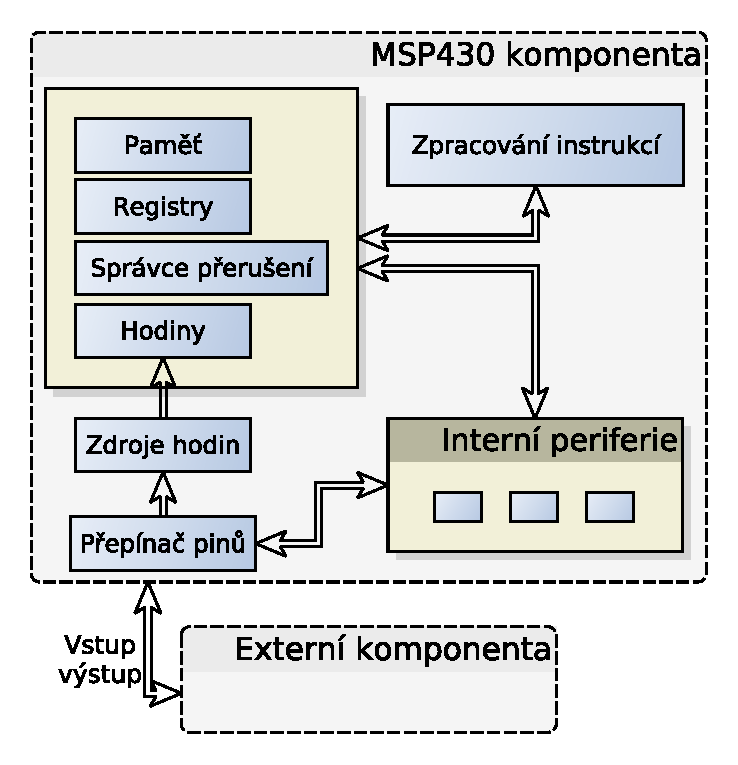
\includegraphics[trim=0cm 0cm 0cm 0cm, scale=0.7]{fig/msp430_arch}
\caption{Návrh architektury MSP430 komponenty.}
\label{fig:msp430_arch}
\end{figure}

\subsection{Paměť}

Paměť slouží k uchování jak uživatelského programu tak dat. Ostatní části mikrokontroléru (zejména pak interní periferie jako například USI nebo USCI) musí být schopny do paměti zapisovat jak slova tak jednotlivé byty a být informovány o případném čtení nebo zápisu provedeném uživatelským programem. To je podstatná vlastnost například pro automatické smazání příznaku přerušení po jeho přečtení. Dalším možným využitím informování zápisu do paměti je možnost zastavení simulace po změně hodnoty v paměti a tím lepší možnost ladit uživatelský program.

\subsection{Registry}

Registry jsou 16 bitové a mikrokontroler MSP430 jich obsahuje 16. Návrh registrů, podobně jako návrh paměti, počítá s možností čtení a zápisu jednoho nebo dvou bytů. Opět je potřeba umožnit ostatním částem mikrokontroléru zjistit, že došlo k zápisu do registru. Typickým předpokládaným využitím je krokování
programu na základě PC registru.

\subsection{Přepínač pinů}

Každá varianta mikrokontroleru obsahuje různé interní periferie a tím pádem i jiný počet pinů a jejich rozmístění. Na jeden pin může být zapojeno více interních periferií a to, která periferie právě daný pin obsluhuje, je určeno na základě registrů (například PxSEL a PxSEL2).

Každá varianta mikrokontroleru MSP430 bude z hlediska pinů a jejich připojení na interní periferie popsána v XML souboru, který bude obsahovat o každém
pinu následující informace:

\begin{itemize}
\item Umístění pinu na pouzdru mikrokontroleru (vlevo, vpravo, ...) včetně jeho pořadí na dané straně pouzdra.
\item Seznam názvů vstupů/výstupu realizovaných pomocí pinu a hodnoty bitů v registrech určujících, který vstup/výstup bude kdy zvolen.
\end{itemize}


Interní komponenty budou mít zaregistrovány v přepínači pinů názvy svých vstupů a výstupů.
Přepínač pinů pak bude na základě aktuální simulované varianty monitorovat registry PxSEL, PxSEL2, ... a na základě jejich hodnoty přeposílat vstupy z externích komponent konkrétním interním periferiím (princip multiplexoru). Tento princip lze vidět na obrázku \ref{fig:msp430_pinmult}.

\begin{figure}[h]
\centering
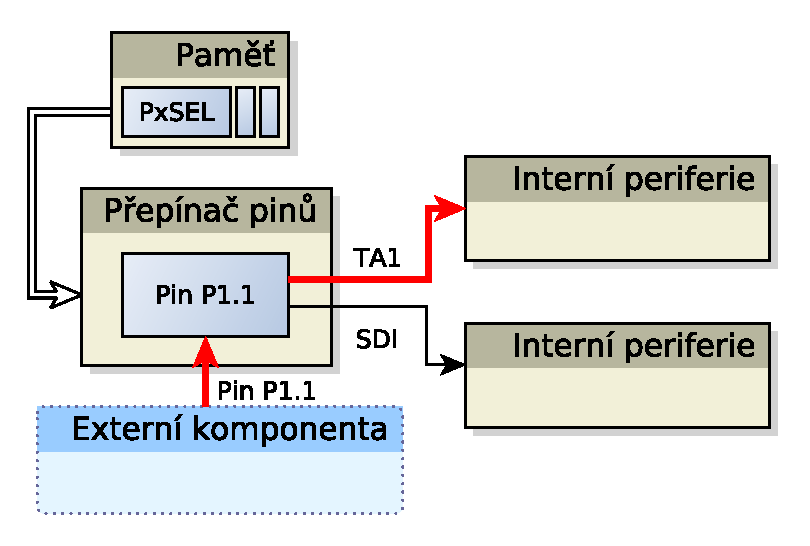
\includegraphics[trim=0cm 0cm 0cm 0cm, scale=0.7]{fig/msp430_pinmult}
\caption{Přepínač pinů přeposílá vstup z externí komponenty na interní periferii podle hodnoty PxSEL.}
\label{fig:msp430_pinmult}
\end{figure}

Přepínač pinů bude rovněž směrovat signály uvnitř MSP430 komponenty. Typickým použitím této vlastnosti bude interní propojení jednotlivých interních periferií (Například výstup časovače může být použit jako vstup modulu USI).

\subsection{Zdroje hodin}

Z hlediska simulace je možné zdroje hodin rozdělit na dvě kategorie. Zdroje závislé na externích komponentách (LFXT1CLK, XT2CLK) a zdroje závislé pouze na čase (VLOCLK, DCOCLK).

Zdroje závislé na externích komponentách musí být schopny přijímat zprávy od externích komponent a na jejich základě pak generovat hodinový signál, který je dále zpracován jednotlivými hodinami.

Zdroje závislé na čase musí být samostatnými simulačními (DEVS) komponentami a musí samy
na základě uběhnutého času generovat hodinový signál s patřičnou frekvencí.

Všechny zdroje hodin musí generovat informace jak o náběžné, tak o sestupné hraně hodinového signálu. To je podstatná vlastnost například pro modul USI, který provádí své akce jak s náběžnou tak sestupnou hranou.

\subsection{Hodiny}

Hodiny (MCLK, SMCLK a ACLK) dále zpracovávají hodinový signál od zdrojů hodinového signálu. Umožňují nastavit děličku, čímž mění frekcenci hodinového signálu. K jednotlivým hodinám jsou pak připojeny periferi, které jsou hodinami řízeny. Stejně jako u zdrojů hodinového signálu je potřeba u zdrojů hodin
poskytovat informace jak o náběžné tak o sestupné hraně.

\subsection{Správce přerušení}

Správce přerušení bude udržovat informace o požadavcích na přerušení. Modulu zpracovávajícímu instrukce umožní spustit rutinu přerušení, pokud je nějaké
přerušení ve frontě. Ostatním periferiím pak umožní žádat o přerušení.

Periferie budou rovněž vyžadovat informaci o dokončení konkrétního typu přerušení (například vymazání indikátoru přerušení po jeho obsluze).

\subsection{Zpracování instrukcí}

Zpracování instrukcí ilustruje diagram na obrázku \ref{fig:msp430_inst}.

\begin{figure}[h]
\centering
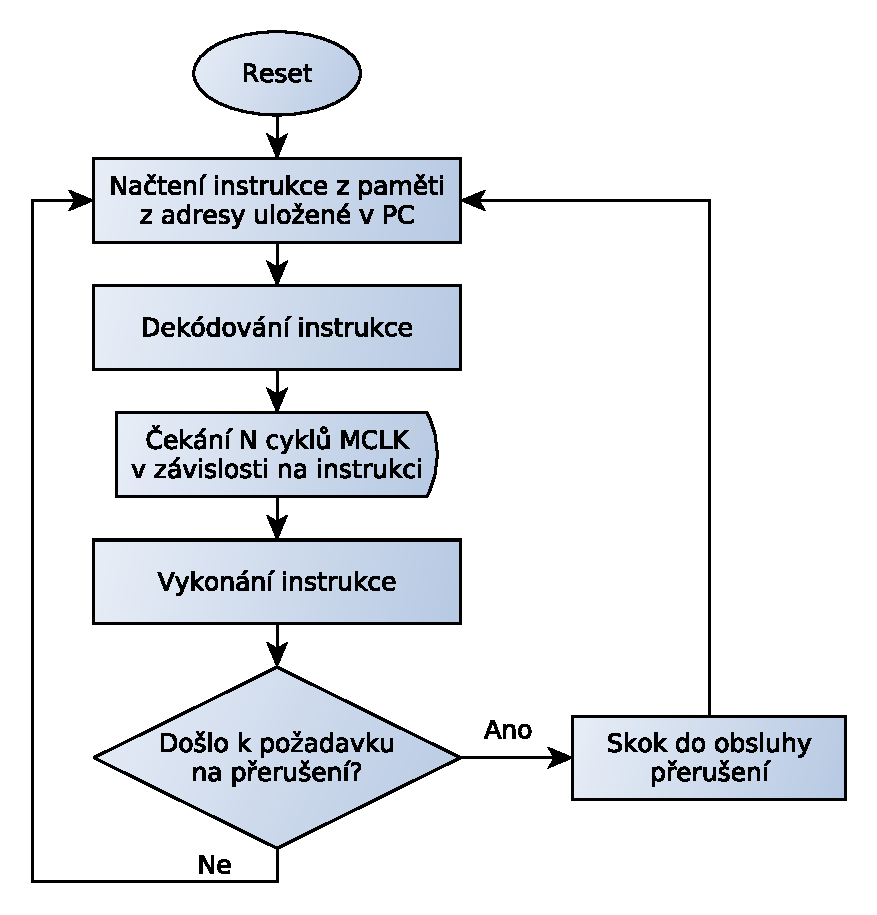
\includegraphics[trim=0cm 0cm 0cm 0cm, scale=0.7]{fig/msp430_inst}
\caption{Diagram zpracování instrukcí.}
\label{fig:msp430_inst}
\end{figure}

Z obrázku lze vidět, že je zpracování instrukce rozděleno na několik částí. Nejprve je instrukce načtena z paměti v závislosti na hodnotě registru PC (R0).
Dále dojde k dekódování instrukce a jejímu vykonání. Vykonání instrukce je atomické a trvá několik MCLK cyklů. Počet cyklů potřebných pro vykonání
instrukce víme již po jejím dekódování. Proto je mezi dekódováním a vykonáním vloženo čekání simulující vykonávání instrukce na reálném HW.
Po vykonání instrukce je potřeba obsloužit jakákoliv přerušení, která mohla v mezičase nastat. Tento cyklus se bude opakovat stále dokola, dokud MCLK generuje další pulsy (tzv. dokud simulace běží).

\subsection{Interní periferie}

Interní periferi budou využívat modulů popsaných dříve v této kapitole. Každá interní perifer tak bude mít přístup k paměti, registrům, pinům, správci
přerušení a hodinovému signálu. V rámci diplomové práce bude z interních periferií implementován časovač, modul USI a USCI.

Jako příklad návrhu interní periferie se tato podkapitola věnuje pouze časovači. Princip návrhu ostatních periferií je však obdobný, liší se pouze jejich funkcí.

\subsubsection{Časovač}

Časovač bude monitorovat své registry prostřednictvím paměťového modulu a v případě jejich změny, způsobené uživatelským programem, změní také své nastavení
(výběr módu, vstupů atd.). Pro generování nastavení Capture overflow bitu (indikace situace, kdy uživatelský program nestihl přečíst hodnotu časovače během 2 přerušení) je potřeba informace, zda uživatelský program přečetl aktuální hodnotu časovače. To bude řešeno opět pomocí paměťového modulu, kdy tento bude informovat časovač o přečtení dané hodnoty z paměti.

Časovač musí být schopen zvyšovat svoji hodnotu v závislosti na frekvenci. Proto bude časovač napojen na modul hodin (SMLK nebo ACLK). Z každým cyklem
hodin pak v závislosti na svém nastavení vykoná danou funkci.

Pomocí časovače lze rovněž generovat pulsy na výstupních pinech umístěných na pouzdře mikrokontroleru a reagovat na změnu napětí na pinech vstupních.
Je proto nutné umožnit časovači přístup k těmto pinům. To bude provedeno pomocí přepínače pinů. Časovač si zaregistruje potřebné názvy vstupů a výstupů
a přepínač pinů pak v závislosti na akcích uživatelského programu bude směrovat vstupy mikrokontroleru přímo do časovače.

Přerušení časovače jsou generována pomocí správce přerušení. Je však potřeba zajistit, aby se časovač dozvěděl o dokončení rutiny obsluhující přerušení
(přerušení časovače je sdíleno více zdroji přerušení a časovač musí být schopen požádat o další přerušení z jiného zdroje ihned po obsloužení původního přerušení). Toto je zajištěno monitorováním ukončených přerušení pomocí správce přerušení.

Z příkladu časovače lze vidět, že návrh a dekompozice mikrokontroleru MSP430 je dostačující pro interní periferie a poskytuje všechny potřebné vlastnosti.


\section{Návrh grafického uživatelského rozhraní}

Hlavní funkcí grafického uživatelského rozhraní je řízení simulace, jednoduchá editace jednotlivých simulovaných komponent a lazení programu mikrokontroleru.

Grafické uživatelské rozhraní by tedy mělo mít následující funkce:

\begin{itemize}
\item \textbf{Správa projektu} - Vytvoření, uložení a nahrání projektu.
\item \textbf{Editace projektu} - Přidávání a odebírání simulovaných komponent a editace jejich propojení.
\item \textbf{Řízení simulace} - Nastavení parametrů simulace, kontrola jejího běhu, krokování atd.
\item \textbf{Lazení programu} - Zobrazení zdrojového kódu programu, hodnoty proměnných, registrů, paměti.
\item \textbf{Lazení signálů} - Možnost kontrolovat v čase signály přenášené mezi simulovanými komponentami.
\end{itemize}

V této kapitole jsou tyto požadavky kladené na grafické uživatelské rozhraní detailně rozebrány a je navženo grafické uživatelské rozhraní, které tyto
požadavky splňuje.

